\documentclass[a4paper]{article}
\usepackage[spanish]{babel}
\usepackage[utf8]{inputenc}
\usepackage{float}
\usepackage{graphicx}
%\usepackage[american voltage]{circuitikz}
\usepackage{amsmath}
\usepackage{xcolor}
\usepackage{caption}
\usepackage{subcaption}
\usepackage[bottom]{footmisc}


\begin{document}
	\subsection{Introducción}
	Los amplificadores de instrumentación, también conocidos como \textbf{IN-AMP},  son utilizados para amplificar con alta precisión las señales provenientes de diversas unidades de adquisición de datos que no poseen la amplitud suficiente como para poder ser aprovechada siendo muy susceptible a contaminación por ruido . Sin embargo, amplificar no es el único objetivo de este dispositivo. Si así fuese entonces bastaría con utilizar un amplificador operacional corriente.
	\subsubsection{Diferencias entre \textbf{IN-AMP} y \textbf{OP AMP}}
	A simple vista, un \textbf{IN-AMP} puede ser fácilmente confundido con un \textbf{OP AMP}. Ambos dispositivos amplifican una señal diferencial, poseen una elevada impedancia de entrada y una muy baja impedancia de salida.
	No obstante, podemos notar algunas diferencias fundamentales. En primer lugar para configurar la ganancia a lazo cerrado de un amplificador operacional se debe ajustar mediante resistores de retro-alimentación externos mientras que en un amplificador de instrumentación la ganancia puede venir predefinida por el fabricante o ajustada mediante una \textbf{resistencia externa}.
	En caso de que se desee amplificar una señal diferencial el amplificador de instrumentación eliminara cualquier componente de señal común a ambas entradas como puede ser un offset de continua o simplemente ruido.
	Esto representa una gran ventaja frente a los amplificadores operacionales tradicionales que no están diseñados para eliminar este tipo señales.

	
	\subsection{Análisis teórico}
	El circuito propuesto debajo es una variante de los famosos amplificadores de instrumentación que utilizan 3 amplificadores operacionales
	%Imagen del amplificador de instrumentación con 3 op-amps
	\begin{figure}[H]
		\centering
		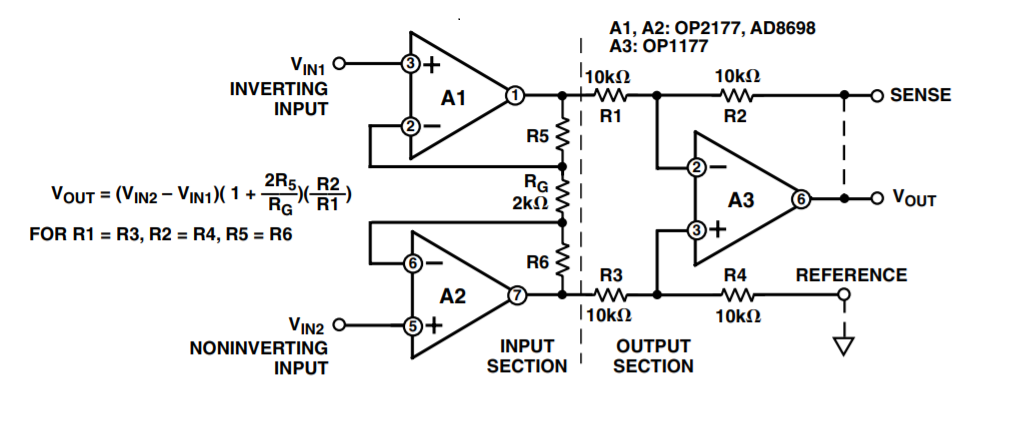
\includegraphics[width=\linewidth]{../ImagenesVarias/inAmp3Opamp}
		\caption[Compact Routing Example]{Clasico amplificador de instrumentación con 3 Opamps }}
	\footnote{Imagen extraída de: \textit{A designer's guide to instrumentation amplifiers}
	\end{figure}


	
	
\begin{thebibliography}{9}
	
	\bibitem{Franco} 
	SERGIO, F. (2002). Design with operational amplifiers and analog integrated circuits. New York [etc.]: McGraw-Hill, pp.73-91.	
	
	\bibitem{Coughlin} 
	R. Coughlin and F. Driscoll, Circuitos integrados lineales y amplificadores operacionales. México: Prentice-Hall Hispanoamericana, 1998.
	
	\bibitem{dguideinamp}
	C. Kitchin and L. Counts, A designer's guide to instrumentation amplifiers. Norwood, Mass.: Analog Devices, 2006.
	
\end{thebibliography}

\end{document}